\documentclass[14pt]{extbook}
\usepackage{multicol, enumerate, enumitem, hyperref, color, soul, setspace, parskip, fancyhdr} %General Packages
\usepackage{amssymb, amsthm, amsmath, latexsym, units, mathtools} %Math Packages
\everymath{\displaystyle} %All math in Display Style
% Packages with additional options
\usepackage[headsep=0.5cm,headheight=12pt, left=1 in,right= 1 in,top= 1 in,bottom= 1 in]{geometry}
\usepackage[usenames,dvipsnames]{xcolor}
\usepackage{dashrule}  % Package to use the command below to create lines between items
\newcommand{\litem}[1]{\item#1\hspace*{-1cm}\rule{\textwidth}{0.4pt}}
\pagestyle{fancy}
\lhead{Progress Quiz 6}
\chead{}
\rhead{Version A}
\lfoot{4563-7456}
\cfoot{}
\rfoot{Summer C 2021}
\begin{document}

\begin{enumerate}
\litem{
Determine the vertical asymptotes and holes in the rational function below.\[ f(x) = \frac{6x^{3} +7 x^{2} -7 x -6}{8x^{2} +2 x -15} \]\begin{enumerate}[label=\Alph*.]
\item \( \text{Vertical Asymptote of } x = 0.75 \text{ and hole at } x = -1.5 \)
\item \( \text{Vertical Asymptotes of } x = 1.25 \text{ and } x = -0.667 \text{ with a hole at } x = -1.5 \)
\item \( \text{Holes at } x = 1.25 \text{ and } x = -1.5 \text{ with no vertical asymptotes.} \)
\item \( \text{Vertical Asymptote of } x = 1.25 \text{ and hole at } x = -1.5 \)
\item \( \text{Vertical Asymptotes of } x = 1.25 \text{ and } x = -1.5 \text{ with no holes.} \)

\end{enumerate} }
\litem{
Determine the vertical asymptotes and holes in the rational function below.\[ f(x) = \frac{9x^{3} -42 x^{2} +16 x + 32}{6x^{2} +7 x -20} \]\begin{enumerate}[label=\Alph*.]
\item \( \text{Vertical Asymptote of } x = -2.5 \text{ and hole at } x = 1.333 \)
\item \( \text{Vertical Asymptotes of } x = -2.5 \text{ and } x = -0.667 \text{ with a hole at } x = 1.333 \)
\item \( \text{Vertical Asymptote of } x = 1.5 \text{ and hole at } x = 1.333 \)
\item \( \text{Vertical Asymptotes of } x = -2.5 \text{ and } x = 1.333 \text{ with no holes.} \)
\item \( \text{Holes at } x = -2.5 \text{ and } x = 1.333 \text{ with no vertical asymptotes.} \)

\end{enumerate} }
\litem{
Which of the following functions \textit{could} be the graph below?
\begin{center}
    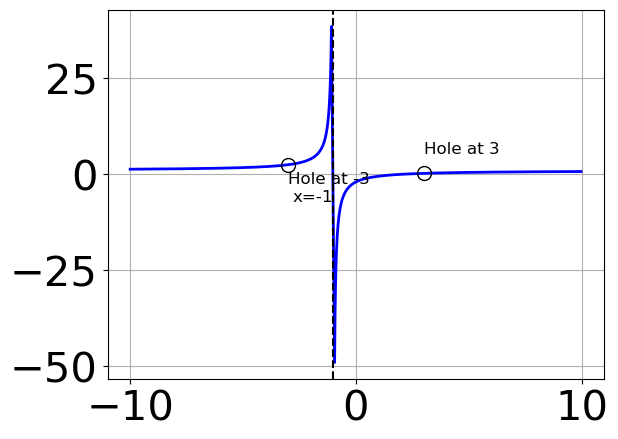
\includegraphics[width=0.5\textwidth]{../Figures/identifyGraphOfRationalFunctionCopyA.png}
\end{center}
\begin{enumerate}[label=\Alph*.]
\item \( f(x)=\frac{x^{3} -10.0 x^{2} +28.0 x -24.0}{x^{3} + x^{2} -9.0 x -9.0} \)
\item \( f(x)=\frac{x^{3} -2.0 x^{2} -9.0 x + 18.0}{x^{3} + x^{2} -9.0 x -9.0} \)
\item \( f(x)=\frac{x^{3} +2.0 x^{2} -25.0 x -50.0}{x^{3} -1.0 x^{2} -9.0 x + 9.0} \)
\item \( f(x)=\frac{x^{3} +2.0 x^{2} -9.0 x -18.0}{x^{3} -1.0 x^{2} -9.0 x + 9.0} \)
\item \( \text{None of the above are possible equations for the graph.} \)

\end{enumerate} }
\litem{
Determine the horizontal and/or oblique asymptotes in the rational function below.\[ f(x) = \frac{12x^{3} -23 x^{2} -22 x + 40}{4x^{2} +3 x -10} \]\begin{enumerate}[label=\Alph*.]
\item \( \text{Horizontal Asymptote of } y = 3.0  \)
\item \( \text{Horizontal Asymptote of } y = -2.0 \text{ and Oblique Asymptote of } y = 3x -8 \)
\item \( \text{Horizontal Asymptote at } y = -2.0 \)
\item \( \text{Horizontal Asymptote of } y = 3.0 \text{ and Oblique Asymptote of } y = 3x -8 \)
\item \( \text{Oblique Asymptote of } y = 3x -8. \)

\end{enumerate} }
\litem{
Determine the horizontal and/or oblique asymptotes in the rational function below.\[ f(x) = \frac{8x^{3} +10 x^{2} -57 x -45}{4x^{2} -17 x -15} \]\begin{enumerate}[label=\Alph*.]
\item \( \text{Horizontal Asymptote of } y = 2.0 \text{ and Oblique Asymptote of } y = 2x + 11 \)
\item \( \text{Horizontal Asymptote of } y = 5.0 \text{ and Oblique Asymptote of } y = 2x + 11 \)
\item \( \text{Horizontal Asymptote at } y = 5.0 \)
\item \( \text{Oblique Asymptote of } y = 2x + 11. \)
\item \( \text{Horizontal Asymptote of } y = 2.0  \)

\end{enumerate} }
\litem{
Determine the horizontal and/or oblique asymptotes in the rational function below.\[ f(x) = \frac{15x^{3} +19 x^{2} -4}{9x^{3} -14 x -8} \]\begin{enumerate}[label=\Alph*.]
\item \( \text{Horizontal Asymptote of } y = 1.667  \)
\item \( \text{Vertical Asymptote of } y = 1.333  \)
\item \( \text{Horizontal Asymptote of } y = 0  \)
\item \( \text{Vertical Asymptote of } y = -1  \)
\item \( \text{None of the above} \)

\end{enumerate} }
\litem{
Determine the vertical asymptotes and holes in the rational function below.\[ f(x) = \frac{12x^{3} -7 x^{2} -30 x + 25}{9x^{2} +27 x + 20} \]\begin{enumerate}[label=\Alph*.]
\item \( \text{Vertical Asymptotes of } x = -1.333 \text{ and } x = -1.667 \text{ with no holes.} \)
\item \( \text{Vertical Asymptote of } x = 1.333 \text{ and hole at } x = -1.667 \)
\item \( \text{Vertical Asymptote of } x = -1.333 \text{ and hole at } x = -1.667 \)
\item \( \text{Vertical Asymptotes of } x = -1.333 \text{ and } x = 1.25 \text{ with a hole at } x = -1.667 \)
\item \( \text{Holes at } x = -1.333 \text{ and } x = -1.667 \text{ with no vertical asymptotes.} \)

\end{enumerate} }
\litem{
Determine the horizontal and/or oblique asymptotes in the rational function below.\[ f(x) = \frac{2x^{2} -x -10}{4x^{3} -12 x^{2} -25 x + 75} \]\begin{enumerate}[label=\Alph*.]
\item \( \text{Horizontal Asymptote of } y = 0.500 \text{ and Oblique Asymptote of } y = 2x -5 \)
\item \( \text{Horizontal Asymptote at } y = -2.000 \)
\item \( \text{Horizontal Asymptote of } y = 0 \)
\item \( \text{Oblique Asymptote of } y = 2x -5. \)
\item \( \text{Horizontal Asymptote of } y = 0.500  \)

\end{enumerate} }
\litem{
Which of the following functions \textit{could} be the graph below?
\begin{center}
    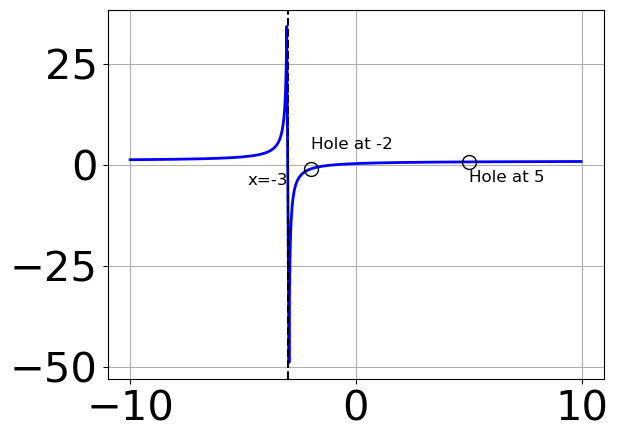
\includegraphics[width=0.5\textwidth]{../Figures/identifyGraphOfRationalFunctionA.png}
\end{center}
\begin{enumerate}[label=\Alph*.]
\item \( f(x)=\frac{x^{3} +4.0 x^{2} -25.0 x -28.0}{x^{3} -19.0 x -30.0} \)
\item \( f(x)=\frac{x^{3} +2.0 x^{2} -13.0 x + 10.0}{x^{3} -19.0 x + 30.0} \)
\item \( f(x)=\frac{x^{3} -2.0 x^{2} -11.0 x + 12.0}{x^{3} -19.0 x + 30.0} \)
\item \( f(x)=\frac{x^{3} -2.0 x^{2} -13.0 x -10.0}{x^{3} -19.0 x -30.0} \)
\item \( \text{None of the above are possible equations for the graph.} \)

\end{enumerate} }
\litem{
Determine the vertical asymptotes and holes in the rational function below.\[ f(x) = \frac{6x^{3} -29 x^{2} +43 x -20}{8x^{2} -26 x + 15} \]\begin{enumerate}[label=\Alph*.]
\item \( \text{Vertical Asymptote of } x = 0.75 \text{ and hole at } x = 2.5 \)
\item \( \text{Vertical Asymptotes of } x = 0.75 \text{ and } x = 2.5 \text{ with no holes.} \)
\item \( \text{Vertical Asymptotes of } x = 0.75 \text{ and } x = 1.333 \text{ with a hole at } x = 2.5 \)
\item \( \text{Holes at } x = 0.75 \text{ and } x = 2.5 \text{ with no vertical asymptotes.} \)
\item \( \text{Vertical Asymptote of } x = 0.75 \text{ and hole at } x = 2.5 \)

\end{enumerate} }
\end{enumerate}

\end{document}